\chapter{Methodology and Simulation Framework}
\label{ch:methodology}

This chapter describes the simulation framework that produced the data analysed in subsequent chapters. We chose simulation over a real-system measurement campaign for three reasons. First, simulation allows complete control over the network topology, message delays and packet loss, all of which are difficult or impossible to vary on physical infrastructure. Second, simulation produces fully reproducible runs through random seeding, which is essential for statistical analysis. Third, simulation isolates the consensus algorithm from confounding factors such as operating system scheduling, garbage collection or hardware interrupts. The trade-off is that the simulator does not capture every nuance of a production deployment; we discuss this limitation explicitly in Chapter~\ref{ch:discussion}.

\section{Design Principles}

The framework was designed around four guiding principles.

\begin{itemize}
    \item \textbf{Faithfulness to Raft:} the simulator implements the leader election and log replication mechanisms described by \citet{ongaro2014} without simplification of the safety-critical parts.
    \item \textbf{Topology agnosticism:} the consensus logic is independent of the underlying topology, which is encapsulated in a separate routing layer. This separation makes it straightforward to add new topologies without modifying the algorithm.
    \item \textbf{Determinism through seeding:} every source of randomness, including election timeouts, message ordering and packet loss, derives from a single configurable random seed. This guarantees that runs are bit-for-bit reproducible.
    \item \textbf{Observability:} every state transition, RPC and log change is recorded as an event, which allows the entire run to be replayed and analysed offline.
\end{itemize}

\section{Architecture}

The simulator is a tick-driven discrete-event system. Time advances in discrete units called \emph{ticks}. At each tick the engine executes a fixed sequence of actions: it delivers messages whose delivery time has arrived, advances the local clock of each node, lets each node process its inbox and produce output messages, and records any state changes in the event log.

The high-level structure consists of a simulation engine that drives a collection of \texttt{Node} objects. Each node owns its persistent state (current term, voted-for, log) and its volatile state (commit index, last applied, role). Communication between nodes is mediated by the \texttt{Network} object, which inspects the topology graph, computes the shortest path between sender and receiver, applies the configured per-hop delay and probabilistically drops messages with the configured loss rate.

\subsection{Engine Loop}

The main loop is conceptually simple. It runs for a configurable number of ticks (the default is 1000) or until a configurable convergence condition is met. Each iteration performs the following:

\begin{enumerate}
    \item Increment the current tick.
    \item Deliver all messages whose scheduled arrival time matches the current tick.
    \item For each non-failed node, advance its local clock and execute its state-machine step.
    \item Schedule any new outgoing messages produced by the nodes.
    \item Record the event log entries produced during the tick.
    \item Optionally inject failures or recoveries based on the configured probabilities.
\end{enumerate}

Because the engine is single-threaded, there are no race conditions; every step is deterministic given the same seed and the same configuration.

\subsection{Node State Machine}

Each node is implemented as a finite state machine with three roles (Follower, Candidate, Leader) and the persistent and volatile state mandated by the Raft specification. The implementation handles the four RPC types: \texttt{RequestVote}, \texttt{RequestVoteResponse}, \texttt{AppendEntries} and \texttt{AppendEntriesResponse}. Heartbeats are realised as empty \texttt{AppendEntries} RPCs.

Election timeouts are sampled from a uniform distribution that, in tick units, corresponds to the range typically used in production Raft deployments. Heartbeat intervals are configured to be roughly a third of the lower bound of the election-timeout range, which is the recommended ratio in the original paper \citep{ongaro2014}. The exact tick parameters used in the experiments are reported in Table~\ref{tab:tick_params}.

\begin{table}[H]
\centering
\caption{Default time parameters of the simulator (in ticks).}
\label{tab:tick_params}
\begin{tabular}{ll}
\toprule
\textbf{Parameter} & \textbf{Value} \\
\midrule
Election timeout (lower bound) & 150 \\
Election timeout (upper bound) & 300 \\
Heartbeat interval             & 50 \\
Default message delay (per hop) & 10 \\
Default simulation duration    & 1000 \\
\bottomrule
\end{tabular}
\end{table}

\subsection{Network Layer}

The network layer is responsible for delivering messages between nodes and for modelling the topology. A topology is represented internally as an adjacency list. Each topology generator builds the corresponding graph for a given number of nodes:

\begin{itemize}
    \item \textbf{Star:} node 0 is the hub; nodes $1$ through $n-1$ are connected only to the hub.
    \item \textbf{Ring:} node $i$ is connected to nodes $(i-1) \bmod n$ and $(i+1) \bmod n$.
    \item \textbf{Mesh:} for every pair $(i, j)$ with $i \neq j$, an edge is created.
    \item \textbf{Tree:} node $i$ has children $2i+1$ and $2i+2$ when those indices exist.
    \item \textbf{Bus:} node $i$ is connected to $i-1$ and $i+1$ when those indices exist.
\end{itemize}

When a node sends a message to another node, the network computes the shortest path between them using a breadth-first search and assigns the message a delivery tick equal to \texttt{current\_tick + (hops $\times$ message\_delay)}. The simulator caches shortest paths to avoid recomputation; the cache is invalidated only when nodes fail or recover, since failures alter the routing graph.

Packet loss is applied per hop: if the configured loss rate is $p$, then for a message that traverses $h$ hops the probability that the message is delivered is $(1-p)^h$. Dropped messages are recorded but not retransmitted at the network layer; retransmission is the responsibility of Raft's own RPC retry logic.

\subsection{Failure Model}

The simulator supports three failure scenarios. The first is per-tick stochastic failure: at every tick, each non-failed node fails with probability $p_f$, and each failed node recovers with probability $p_r$. The second is deterministic injection: a specific node, identified by index or by role (most notably the current leader), can be marked as failed at a configured tick. The third is a combination of the two. Failed nodes drop all incoming messages and produce no outgoing messages until they recover; on recovery, a node is restored to the follower state with whatever persistent state it had at the moment of failure.

\section{Implementation}

The simulator is implemented in Python 3.11 and consists of approximately 950 lines of code split across two main modules.

\begin{itemize}
    \item \texttt{raft\_engine.py}: implements the \texttt{Node}, \texttt{Network} and \texttt{SimulationEngine} classes. The \texttt{SimulationEngine} class exposes a \texttt{run()} method that returns a dictionary containing the metrics, the full event log and the per-tick history.
    \item \texttt{server.py}: a FastAPI application that exposes a REST API for launching simulations, comparing runs, retrieving history and exporting CSV reports. It persists simulation results in a SQLite database via \texttt{aiosqlite}.
\end{itemize}

A complementary React frontend, built with Tailwind CSS and Recharts, provides a real-time dashboard for the experiments. The frontend visualises the network graph as it evolves, displays the live metric values, and allows the user to replay a stored simulation step by step. Although the frontend was useful during development to validate qualitative behaviour, all quantitative data reported in this thesis was produced by direct invocation of the engine rather than through the user interface.

As permitted under the UBB recommendations on AI use in academic writing (HCA no.\ 3961/25.03.2024), which note that for domains involving large data volumes or code generation, generative AI ``is also a standard instrument,'' an AI coding assistant (\textbf{Claude Code, Anthropic, using the Claude Sonnet~4.6 and Claude Opus~4.8 models}) was used throughout development as an auxiliary tool for writing boilerplate code, debugging, refactoring, and generating analysis and plotting scripts for the simulation engine, experiment runner, and dashboard described in this chapter. The simulation architecture, experimental design, and the validation and interpretation of all results remain the author's own work.

\subsection{User Interface}

The frontend exposes the simulator's functionality through three pages. Figure~\ref{fig:ui_dashboard} shows the simulation dashboard: the centre panel renders the network graph for the selected topology, with nodes coloured by their current Raft state (leader, candidate, follower or dead); the left panel exposes the configuration parameters (topology, node count, message delay, packet loss, failure/recovery probabilities, run duration and log entry rate); and the bottom panel reports the resulting metrics alongside charts of messages sent over time, the breakdown of RPC types, and the votes received in each leader election.

\begin{figure}[H]
\centering
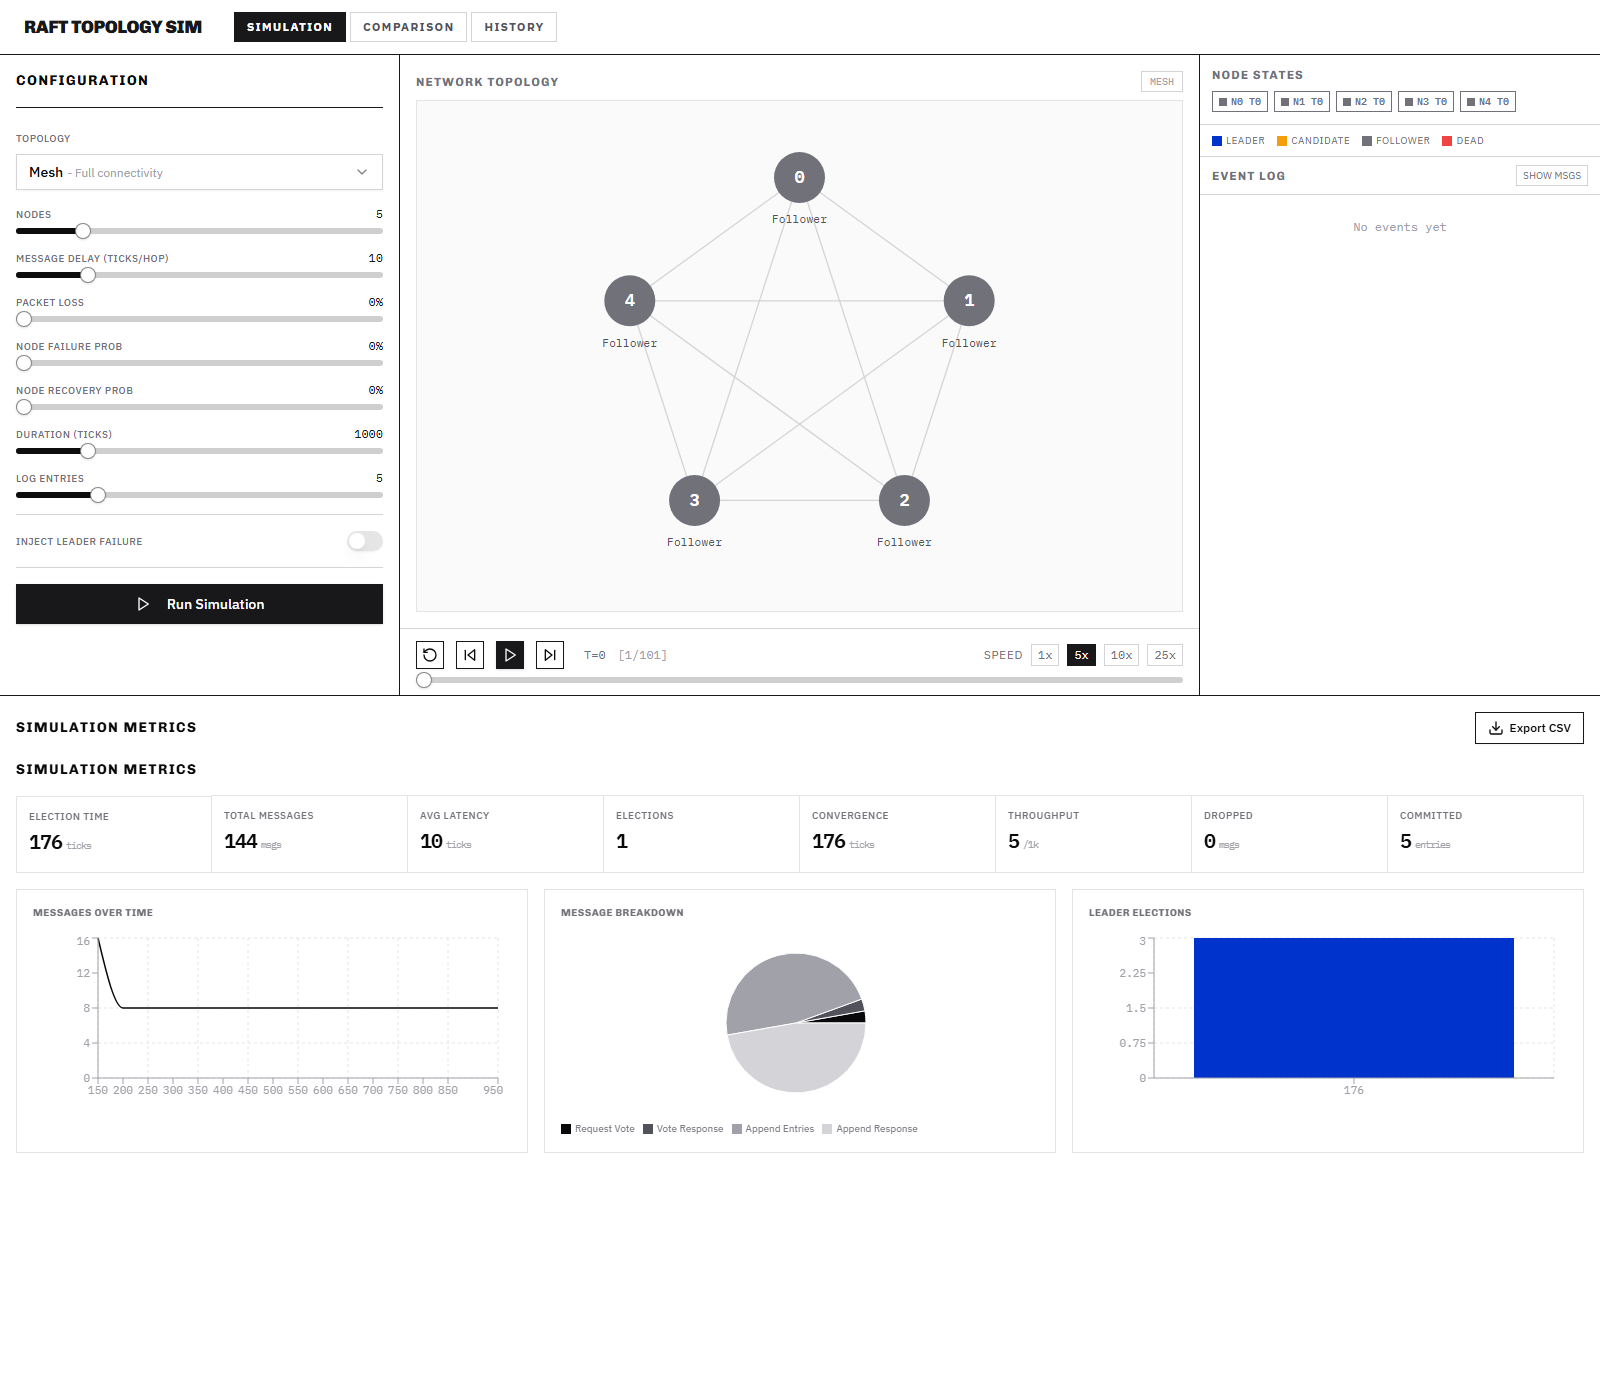
\includegraphics[width=\textwidth]{figures/dashboard.png}
\caption{Simulation dashboard, showing the network topology graph, configuration panel and metric charts for a five-node Mesh run.}
\label{fig:ui_dashboard}
\end{figure}

Figure~\ref{fig:ui_comparison} shows the comparison page, which runs the same configuration across all five topologies and displays the resulting metrics side by side as bar charts and a detailed table -- the same view used to sanity-check the experiment results presented in Chapter~\ref{ch:results}.

\begin{figure}[H]
\centering
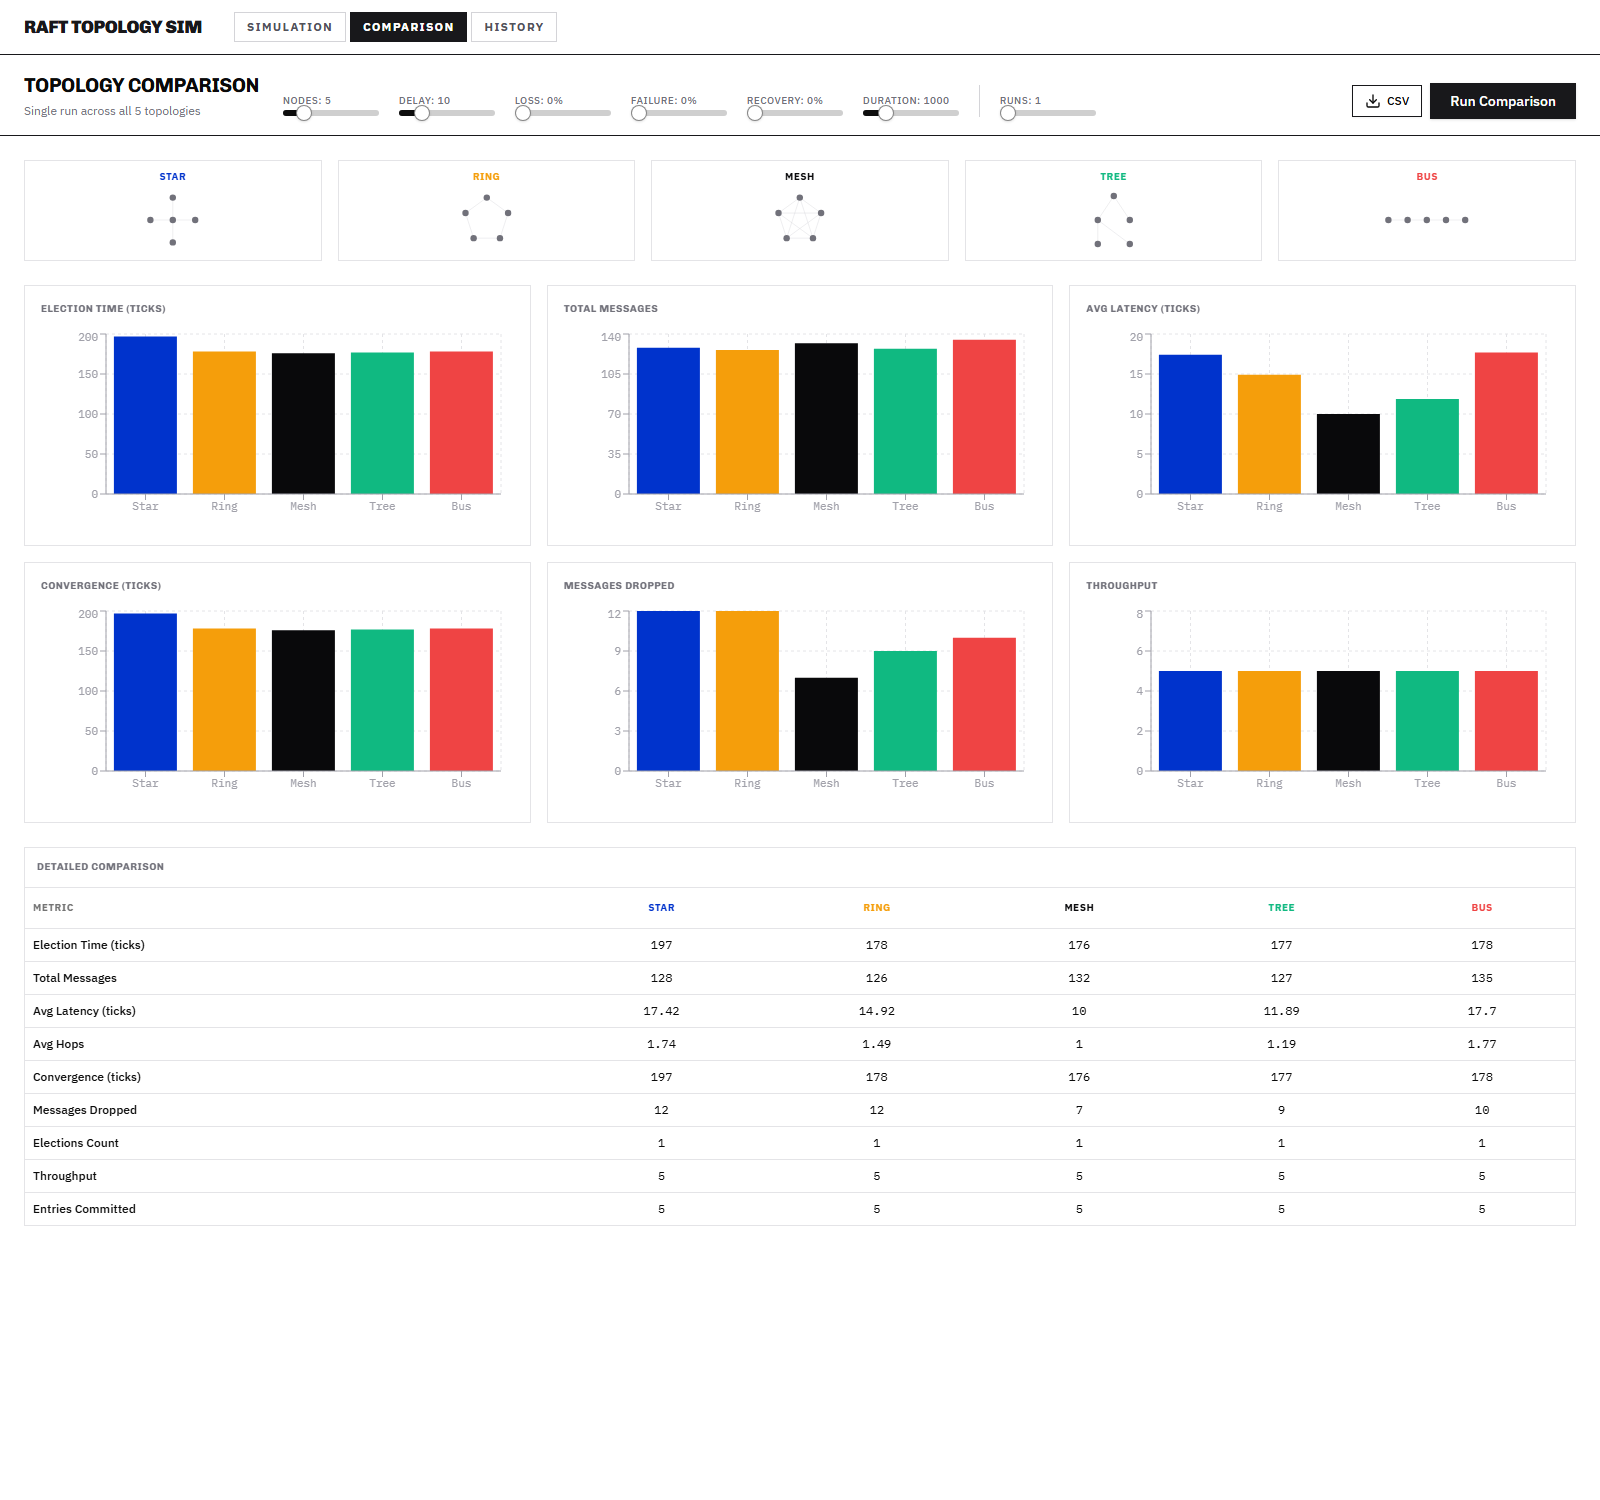
\includegraphics[width=\textwidth]{figures/comparison.png}
\caption{Topology comparison page, showing per-topology bar charts and a detailed metrics table for a single comparison run across all five topologies.}
\label{fig:ui_comparison}
\end{figure}

Figure~\ref{fig:ui_history} shows the history page, which lists previously run simulations together with their key metrics and allows any of them to be replayed.

\begin{figure}[H]
\centering
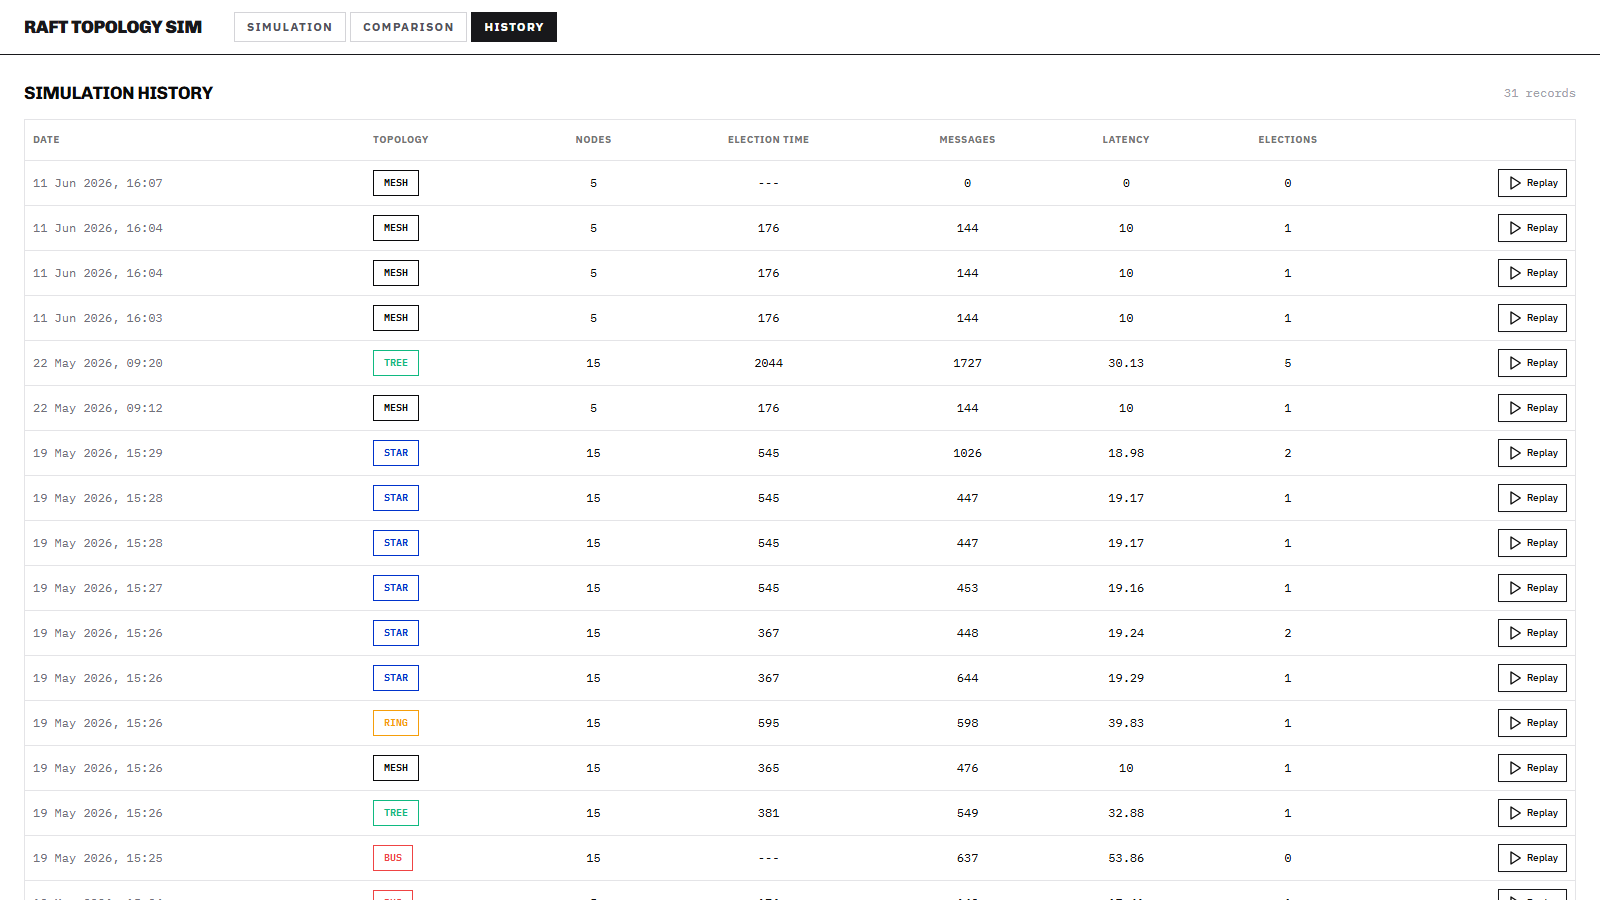
\includegraphics[width=\textwidth]{figures/history.png}
\caption{Simulation history page, listing past runs with their topology, configuration and summary metrics.}
\label{fig:ui_history}
\end{figure}

\section{Metrics}

For each run the simulator records the following metrics. They were chosen to cover the three properties most often discussed in the consensus literature: liveness (how quickly the algorithm makes progress), efficiency (how many resources it consumes) and resilience (how well it copes with failures).

\begin{itemize}
    \item \textbf{First leader election time:} the tick at which the first leader was elected.
    \item \textbf{Convergence time:} the tick at which the cluster reached a steady state, defined as the moment all replicated entries have been committed to a majority.
    \item \textbf{Election count:} the number of distinct leader elections that occurred during the run.
    \item \textbf{Total messages sent:} the cumulative number of RPCs (including heartbeats) issued by all nodes.
    \item \textbf{Total messages dropped:} the cumulative number of RPCs lost to packet loss or to a failed destination.
    \item \textbf{Average latency in hops:} the mean number of hops traversed by delivered RPCs.
    \item \textbf{Average latency in ticks:} the mean delivery delay of RPCs, including hop count and per-hop delay.
    \item \textbf{Throughput:} the number of log entries committed per 100 ticks.
    \item \textbf{Entries committed:} the total number of log entries that reached commit index across the run.
\end{itemize}

\section{Statistical Aggregation}

For each scenario we run the simulation $k$ times with distinct random seeds, where $k$ is between five and ten depending on computational cost. For each metric we compute the mean and the standard deviation across the $k$ runs. We also retain the minimum and maximum to highlight tail behaviour, which is sometimes more revealing than the mean. The aggregation routine is implemented in the helper script \texttt{run\_experiments.py} and produces a single JSON file that drives the analysis presented in Chapter~\ref{ch:results}.

\section{Reproducibility and Validation}

All experiments are reproducible with the seeds and parameters reported in Chapter~\ref{ch:experiments}. We validated the simulator informally in three ways. First, we executed the standard Raft scenarios from the original paper (single-node failure, leader partition) and verified that the outcomes match the expected behaviour. Second, we ran a Mesh topology with zero packet loss and verified that throughput and per-hop message latency are identical regardless of seed, confirming that the algorithm's steady-state behaviour does not depend on the network when it introduces no variance; leader-election time and total message count vary modestly across seeds because each node's election timeout is itself drawn from a per-seed random distribution. Third, we manually inspected event logs from selected runs to confirm that the sequence of state transitions is consistent with the Raft specification.

While these checks do not constitute a formal proof of correctness, they give confidence that the simulator is a reasonable model of Raft's behaviour. Any limitations introduced by the simulation abstraction are discussed in Section~\ref{sec:limitations}.

